%%%%%%%%%%%%%%%%%%%%%%%%%%%%%%%%%%%%%%%%%
% Masters/Doctoral Thesis 
% LaTeX Template
% Version 1.43 (17/5/14)
%
% This template has been downloaded from:
% http://www.LaTeXTemplates.com
%
% Original authors:
% Steven Gunn 
% http://users.ecs.soton.ac.uk/srg/softwaretools/document/templates/
% and
% Sunil Patel
% http://www.sunilpatel.co.uk/thesis-template/
%
% License:
% CC BY-NC-SA 3.0 (http://creativecommons.org/licenses/by-nc-sa/3.0/)
%
% Note:
% Make sure to edit document variables in the Thesis.cls file
%
%%%%%%%%%%%%%%%%%%%%%%%%%%%%%%%%%%%%%%%%%

%----------------------------------------------------------------------------------------
%	PACKAGES AND OTHER DOCUMENT CONFIGURATIONS
%----------------------------------------------------------------------------------------

\documentclass[11pt, oneside]{Thesis} % The default font size and one-sided printing (no margin offsets)

\graphicspath{{Pictures/}} % Specifies the directory where pictures are stored

\usepackage[square, numbers, comma, sort&compress]{natbib} % Use the natbib reference package - read up on this to edit the reference style; if you want text (e.g. Smith et al., 2012) for the in-text references (instead of numbers), remove 'numbers' 
\hypersetup{urlcolor=black, colorlinks=true} % Colors hyperlinks in blue - change to black if annoying
\title{\ttitle} % Defines the thesis title - don't touch this

\begin{document}

\frontmatter % Use roman page numbering style (i, ii, iii, iv...) for the pre-content pages

\setstretch{1.3} % Line spacing of 1.3

% Define the page headers using the FancyHdr package and set up for one-sided printing
\fancyhead{} % Clears all page headers and footers
\rhead{\thepage} % Sets the right side header to show the page number
\lhead{} % Clears the left side page header

\pagestyle{fancy} % Finally, use the "fancy" page style to implement the FancyHdr headers

\newcommand{\HRule}{\rule{\linewidth}{0.5mm}} % New command to make the lines in the title page

% PDF meta-data
\hypersetup{pdftitle={\ttitle}}
\hypersetup{pdfsubject=\subjectname}
\hypersetup{pdfauthor=\authornames}
\hypersetup{pdfkeywords=\keywordnames}

%----------------------------------------------------------------------------------------
%	TITLE PAGE
%----------------------------------------------------------------------------------------

\begin{titlepage}
\begin{center}

\textsc{\LARGE \univname}\\[1.5cm] % University name


\includegraphics[scale=0.4]{logo.png}

\textsc{\Large Bachelor Thesis}\\[0.5cm] % Thesis type

\HRule \\[0.4cm] % Horizontal line
{\huge \bfseries \ttitle}\\[0.4cm] % Thesis title
\HRule \\[1.5cm] % Horizontal line
 
\begin{minipage}{0.4\textwidth}
\begin{flushleft} \large
\emph{Author:}\\
\href{http://www.johnsmith.com}{\authornames} % Author name - remove the \href bracket to remove the link
\newline
\newline
\end{flushleft}
\end{minipage}
\begin{minipage}{0.4\textwidth}
\begin{flushright} \large
\emph{Supervisors:} \\
\href{http://www.cs.vu.nl/~kielmann/}{Dr.-Ing. habil. Thilo Kielmann}
\href{https://systems.cs.pub.ro/people/nicolae.tapus/}{Prof. Dr.-Ing. Nicolae Tapus}
\href{}{M.Sc. Alexandru Uta}
\end{flushright}
\end{minipage}\\[3cm]
 
\large \textit{A thesis submitted in fulfilment of the requirements\\ for the degree of \degreename}\\[0.3cm] % University requirement text
\textit{in the}\\[0.4cm]
%\groupname\\
\deptname\\[2cm] % Research group name and department name
 
{\large \today}\\[4cm] % Date
 
\vfill
\end{center}

\end{titlepage}

%----------------------------------------------------------------------------------------
%	DECLARATION PAGE
%	Your institution may give you a different text to place here
%----------------------------------------------------------------------------------------

\Declaration{

\addtocontents{toc}{\vspace{1em}} % Add a gap in the Contents, for aesthetics

I, \authornames, declare that this thesis titled, '\ttitle' and the work presented in it are my own. I confirm that:

\begin{itemize} 
\item[\tiny{$\blacksquare$}] This work was done wholly or mainly while in candidature for a research degree at this University.
\item[\tiny{$\blacksquare$}] Where any part of this thesis has previously been submitted for a degree or any other qualification at this University or any other institution, this has been clearly stated.
\item[\tiny{$\blacksquare$}] Where I have consulted the published work of others, this is always clearly attributed.
\item[\tiny{$\blacksquare$}] Where I have quoted from the work of others, the source is always given. With the exception of such quotations, this thesis is entirely my own work.
\item[\tiny{$\blacksquare$}] I have acknowledged all main sources of help.
\item[\tiny{$\blacksquare$}] Where the thesis is based on work done by myself jointly with others, I have made clear exactly what was done by others and what I have contributed myself.\\
\end{itemize}
 
Signed:\\
\rule[1em]{25em}{0.5pt} % This prints a line for the signature
 
Date:\\
\rule[1em]{25em}{0.5pt} % This prints a line to write the date
}

\clearpage % Start a new page

%----------------------------------------------------------------------------------------
%	QUOTATION PAGE
%----------------------------------------------------------------------------------------

\pagestyle{empty} % No headers or footers for the following pages

\null\vfill % Add some space to move the quote down the page a bit

\textit{``Thanks to my solid academic training, today I can write hundreds of words on virtually any topic without possessing a shred of information, which is how I got a good job in journalism."}

\begin{flushright}
Dave Barry
\end{flushright}

\vfill\vfill\vfill\vfill\vfill\vfill\null % Add some space at the bottom to position the quote just right

\clearpage % Start a new page

%----------------------------------------------------------------------------------------
%	ABSTRACT PAGE
%----------------------------------------------------------------------------------------

\addtotoc{Abstract} % Add the "Abstract" page entry to the Contents

\abstract{\addtocontents{toc}{\vspace{1em}} % Add a gap in the Contents, for aesthetics

The Thesis Abstract is written here (and usually kept to just this page). The page is kept centered vertically so can expand into the blank space above the title too\ldots
}

\clearpage % Start a new page

%----------------------------------------------------------------------------------------
%	ACKNOWLEDGEMENTS
%----------------------------------------------------------------------------------------

\setstretch{1.3} % Reset the line-spacing to 1.3 for body text (if it has changed)

\acknowledgements{\addtocontents{toc}{\vspace{1em}} % Add a gap in the Contents, for aesthetics

The acknowledgements and the people to thank go here, don't forget to include your project advisor\ldots
}
\clearpage % Start a new page

%----------------------------------------------------------------------------------------
%	LIST OF CONTENTS/FIGURES/TABLES PAGES
%----------------------------------------------------------------------------------------

\pagestyle{fancy} % The page style headers have been "empty" all this time, now use the "fancy" headers as defined before to bring them back

\lhead{\emph{Contents}} % Set the left side page header to "Contents"
\tableofcontents % Write out the Table of Contents

\lhead{\emph{List of Figures}} % Set the left side page header to "List of Figures"
\listoffigures % Write out the List of Figures

\lhead{\emph{List of Tables}} % Set the left side page header to "List of Tables"
\listoftables % Write out the List of Tables

%----------------------------------------------------------------------------------------
%	ABBREVIATIONS
%----------------------------------------------------------------------------------------

\clearpage % Start a new page

\setstretch{1.5} % Set the line spacing to 1.5, this makes the following tables easier to read

\lhead{\emph{Abbreviations}} % Set the left side page header to "Abbreviations"
\listofsymbols{ll} % Include a list of Abbreviations (a table of two columns)
{
\textbf{LAH} & \textbf{L}ist \textbf{A}bbreviations \textbf{H}ere \\
%\textbf{Acronym} & \textbf{W}hat (it) \textbf{S}tands \textbf{F}or \\
}

%----------------------------------------------------------------------------------------
%	PHYSICAL CONSTANTS/OTHER DEFINITIONS
%----------------------------------------------------------------------------------------

\clearpage % Start a new page

\lhead{\emph{Physical Constants}} % Set the left side page header to "Physical Constants"

\listofconstants{lrcl} % Include a list of Physical Constants (a four column table)
{
Speed of Light & $c$ & $=$ & $2.997\ 924\ 58\times10^{8}\ \mbox{ms}^{-\mbox{s}}$ (exact)\\
% Constant Name & Symbol & = & Constant Value (with units) \\
}

%----------------------------------------------------------------------------------------
%	SYMBOLS
%----------------------------------------------------------------------------------------

\clearpage % Start a new page

\lhead{\emph{Symbols}} % Set the left side page header to "Symbols"

\listofnomenclature{lll} % Include a list of Symbols (a three column table)
{
$a$ & distance & m \\
$P$ & power & W (Js$^{-1}$) \\
% Symbol & Name & Unit \\

& & \\ % Gap to separate the Roman symbols from the Greek

$\omega$ & angular frequency & rads$^{-1}$ \\
% Symbol & Name & Unit \\
}

%----------------------------------------------------------------------------------------
%	DEDICATION
%----------------------------------------------------------------------------------------

\setstretch{1.3} % Return the line spacing back to 1.3

\pagestyle{empty} % Page style needs to be empty for this page

\dedicatory{To my Mother, Father and Sister\ldots} % Dedication text

\addtocontents{toc}{\vspace{2em}} % Add a gap in the Contents, for aesthetics

%----------------------------------------------------------------------------------------
%	THESIS CONTENT - CHAPTERS
%----------------------------------------------------------------------------------------

\mainmatter % Begin numeric (1,2,3...) page numbering

\pagestyle{fancy} % Return the page headers back to the "fancy" style

% Include the chapters of the thesis as separate files from the Chapters folder
% Uncomment the lines as you write the chapters

% Chapter 1

\chapter{Introduction} % Main chapter title

\label{Chapter1} % For referencing the chapter elsewhere, use \ref{Chapter1} 

\lhead{Chapter 1. \emph{Introduction}} % This is for the header on each page - perhaps a shortened title

%----------------------------------------------------------------------------------------

Many-Task Computing (MTC)\cite{mtc} is a new computing paradigm that attempts to place itself in-between High-Throughput Computing (HTC) and High-Performance Computing (HPC). The core idea of MTC is that it uses large amounts of computing resources over short periods of time, in order to complete multiple tasks. While a common metric in HTC is the number of tasks fulfilled per month, MTC is usually quantified in tasks per second. Also, as opposed to other paradigms that use message passing as a way to communicate between successive steps in a computation, MTC couples its compute phases via files. Because of this, another common metric of MTC is megabytes per second (MB/s).

Any computing task that is comprised of multiple small parallel jobs is a good fit for MTC. Multiple applications have been found good fits for MTC\cite{mtc}, spanning domains like astronomy, astrophysics, economic modelling, pharmaceutics, chemistry, bioinformatics, neuroscience, data analytics, data mining and biometrics.

MTC exhibits a specific set of technical particularities which need to be properly supported in order to obtain good performance. The high number of parallel tasks that need to be executed underlines the importance of a streamlined scheduling system. Besides that, the way the tasks use files to communicate makes the overall performance largely dependant on the underlying filesystem performance. For the purpose of our subject, we will focus on the filesystem aspect.

% TODO <diagram with tasks using files storing data and then new tasks using that data>

Typically, MTC jobs are run on clusters of compute nodes. These compute nodes need to share data files between them in order to complete the tasks that are assigned to them. Usually, files are locally stored on disk drives (either mechanical disk drives or solid state drives), and get sent over the network when a different node needs access. However, even with the fastest drives commercially available today, the transfer rates of disk drives are inferior to the bandwidth of InfiniBand connections that are used in clusters, considering the fact that a SATA link tops out at 3 GBps while InfiniBand 12X supports a 30 GBps data link. This shows that the bottleneck is not the network, but the storage technology. To overcome this bottleneck, RAM can be used as a storage medium. Obviously it cannot achieve the same storage capacity as regular disk drives, but that is not a problem for the purposes of MTC, as the data files used are not so large in size.

In order to make use of the high speed RAM and network connections that compute nodes in today's clusters have, research groups have started work on developing distributed, in-memory filesystems. These filesystems are specifically designed to support MTC workloads and yield better results than common network filesystems like NFS.

% TODO <diagram showing that amfs/memfs is better than nfs>

To illustrate how such filesystems work, we will describe two implementations - AMFS\cite{amfs} and MemFS\cite{memfs}.

** memfs
** amfs

% TODO - discuss the two filesystems

** why benchmarking them is different (access patterns) - explicit
% Chapter Template

\chapter{Background and Related Work} % Main chapter title

\label{Chapter2} % Change X to a consecutive number; for referencing this chapter elsewhere, use \ref{ChapterX}

\lhead{Chapter 2. \emph{Background and Related Work}} % Change X to a consecutive number; this is for the header on each page - perhaps a shortened title


As we outlined in the Introduction, distributed MTC filesystems are inherently different when compared to usual filesystems. Thus, they have to be benchmarked differently. The relevant set of metrics that needs to be measured is defined in the MTC Envelope\cite{envelope}. It includes the following:

\begin{itemize}

\item file open operation throughput
\item file creation operation throughput
\item 1-to-1 read data throughput
\item 1-to-1 read data bandwidth
\item N-to-1 read data throughput
\item N-to-1 read data bandwidth
\item write data throughput
\item write data bandwidth

\end{itemize}

In the above list, we can observe two special access patterns, specific to MTC filesystems: 1-to-1 and N-to-1 reads.

The 1-to-1 access pattern can be described as follows. There is created a number \textit{N} of files. Then, the \textit{M} nodes each read $N / M$ of the files. Thus, every node has to do with its own set of files and there is no concurrent access over any one file.

The N-to-1 access pattern is a bit more involved. There is only one file created, and then all \textit{M} nodes read it, concurrently. This pattern generates contention and is more penalizing on the performance of the filesystem.

Overall, there are already a significant number of filesystem benchmarks available\cite{fsbench}. However, none of them is a good fit on its own for benchmarking MTC filesystems. We outline a few sample reasons.

Most filesystem benchmarks target disk-based filesystems. This does not fit MTC filesystems because they use RAM as datastore, for performance reasons. The differences between RAM and disks make regular benchmarks unreliable. For example, memory is random access, while disk drives favor sequential access. The difference in access patterns yields less relevant results overall.

Generally, filesystem benchmarks are local - they run on a single node, just like the filesystem implementations they commonly test. This means that in order to run a benchmark on a distributed filesystem, one has to copy the executable on all nodes, run it simultaneously and then aggregate all the results. This approach is tedious, requiring a lot of extra work that is unrelated to the research problem. Furthermore, this way of running tests is not necessarily correct. For example, if an N-to-1 pattern is tested, the N readers should access the file all at the same time. To obtain this, a global synchronization mehtod, such a barrier, should be used. This synchronization cannot be reached by just using a shell script. This means that different test runs will output different results.

However, we can build upon such existing benchmarks. For our solution, we chose to use \textit{IOzone}\cite{iozone} and \textit{mdtest}\cite{mdtest}.


IOzone is a benchmark for measuring I/O performance. It can generate multiple types of file operations, as well as measure their performance. The main operations that are useful for our purposes are:

\begin{itemize}
\item read
\item write
\item re-read
\item re-write
\end{itemize}

Other operations like random read and random write are supported as well, but they are not relevant for memory-based filesystems.

A big advantage of IOzone is that it is written in ANSI C, using POSIX APIs. Because of this, IOzone has been ported to run on multiple computer platforms. It also supports large files in its test runs, which helps in simulating MTC-sized data files.

Another useful feature of IOzone that made embedding it into our benchmark easier is the fact that it can output its results in tab-separated columns, making the results easy to parse.

Below are a subset of the configuration options IOzone supports.

\begin{itemize}

\item cache line size
\item total cache size
\item record size
\item file size
\item including the \textit{close} operation in the timing
\item including flush operations (\textit{fsync}, \textit{fflush}) in the timing
\item performing synchronized writes
\item give results in operations per second
\item purging the CPU cache before each operation

\end{itemize}

While IOzone is a great tool for benchmarking the throughput of reads and writes, we turned to mdtest for benchmarking metadata operations. \textit{mdtest}\cite{mdtest} is a filesystem metadata benchmark that works as follows - first, it creates a file structure (directories and trees) and then it measures performance of operations like \textit{open}, \textit{stat} and \textit{close} on that file structure.

\textit{mdtest} is highly configurable, supporting options like:

\begin{itemize}

\item branching factor of the created file tree
\item number of iterations
\item number of files created within a directory
\item restrict to only measuring one operation (i.e. read)

\end{itemize}

On top of these, mdtest is already a distributed benchmark through the use of MPI. This means that we can use mdtest out of the box to benchmark metadata operations on MTC filesystems. However, there is still room for improvement, especially in the results aggregation and plotting. The benchmark's results are not presented in a machine-readable format, and that means there is no easy way to feed them into a plotting tool. To overcome this, one can use a parser that transforms mdtest output into structured data, like a JSON file.

% Chapter Template

\chapter{A Benchmark for MTC Filesystems} % Main chapter title

\label{Chapter3} % Change X to a consecutive number; for referencing this chapter elsewhere, use \ref{ChapterX}

\lhead{Chapter 3. \emph{A Benchmark for MTC Filesystems}} % Change X to a consecutive number; this is for the header on each page - perhaps a shortened title

In the previous two chapters we have discussed about Many-Task Computing, how it is relevant for today's  computations and why it needs special filesystems. We looked at how those filesystems differ from regular disk-based ones, as well as why they need to be benchmarked differently. We also outlined the shortcomings of current benchmarks and how they can be surpassed. In this chapter, we focus on our approach to building an MTC-specific filesystem benchmark, the architecture behind it and the ways in which it can be used.

\section{Running coordinated commands across multiple nodes}\label{sec:coordination}

As we previously explained, in order to correctly benchmark access patterns on distributed filesystems, all nodes have to start running any given operation simultaneously. To solve this, we need to have a way of synchronizing nodes. Fortunately, synchronization is a common problem with multiple solutions in distributed programming frameworks.

To solve this problem, we used OpenMPI\cite{openmpi} barriers. We developed an MPI application that executes any given command on a set of available nodes. To do so, we spawn MPI workers in the default shared MPI communicator, we then synchronize them with the use of a barrier, and then the workers run the given command. By using the barrier, we can be sure that the command is run in a coordinated manner, at the same time.


\begin{figure}[H]
  \centering
    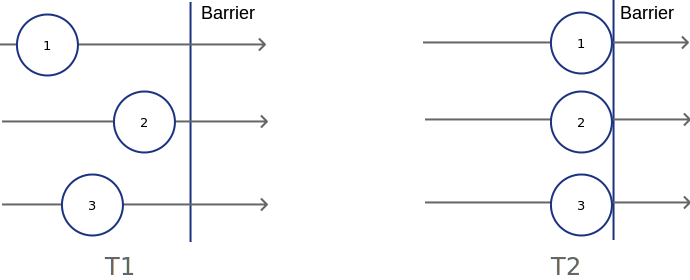
\includegraphics[scale=0.5]{Figures/barrier.png}
    \rule{25em}{0.5pt}
  \caption[MPI barrier]{Synchronizing processes with a barrier}
  \label{fig:barrier}
\end{figure}


% ---------------


\section{Why OpenMPI}

For our solution, we chose to use the MPI framework and, specifically, the OpenMPI\cite{openmpi} implementation. In this subsection we argument why.

Message Passing Interface (MPI) is a standardized communication protocol that is used to implement parallel computations. It defines an API that supports both collective (broadcast, scatter, gather) and point-to-point (send, receive) operations. Our solution makes use of both types of operations. We use a barrier to synchronize the nodes before running the core of the benchmark, and then we use point-to-point operations to send back the output from individual nodes to the master node, which aggregates the results. From our point of view, using MPI has two big advantages.

First, there are implementations available for most of the existing computer architectures existent today\cite{mpi_implementations}. This means that by using standard POSIX and MPI in a program, it can run with no extra porting work on multiple architectures. Since we want our benchmark to be accessible to everybody, portability is a great concern. To achieve this, we made sure to only use standard APIs and to not rely on any implementation-specific behavior in our code.

Second, MPI is built to scale natively. This means that we can write the code for a distributed application once and then run it on any number of nodes without having to change anything. The way this works at the API level is fairly simple - all instances are together in a container (called communicator) and within that container they all have a rank (which is an integer identifier).


Because MPI was implemented for a multitude of different architectures, it is generally supported on computer clusters. We developed our solution on the DAS4\cite{das4} cluster which has support for multiple MPI implementations:

\begin{itemize}

\item OpenMPI
\item MPICH
\item MPICH2
\item Intel MPI

We decided to use OpenMPI mainly because of its open source and vendor-independent nature. However, if OpenMPI is not available for some users of our benchmark, they can use any other implementation without problems, as our code relies only on standard behavior.

\end{itemize}

% ----------

\section{Aggregating the outputs of multiple nodes}

Having an MPI program that runs any given command across multiple nodes, we need a way to capture the outputs and then aggregate them. This is needed because benchmarks like IOzone and mdtest display the performance statistics on the standard output (stdout). Our distributed program has every slave node capture its own output then send it back to the master node, which in turn aggregates all outputs and formats them accordingly.

\begin{figure}[H]
  \centering
    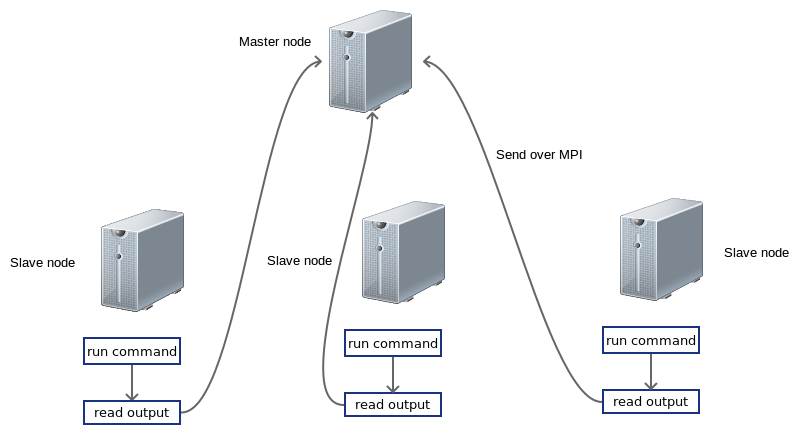
\includegraphics[scale=0.5]{Figures/slave_send_output.png}
    \rule{25em}{0.5pt}
  \caption[Slave nodes sending output]{Slave nodes sending output to master node}
  \label{fig:slave_send_output}
\end{figure}


To solve this problem, our initial solution was to use the \textit{popen}\cite{popen} system call. This runs a given command and captures its output. Then, that output can be sent over MPI to the master node for aggregation. While this approach worked when testing locally using threads, when we tested across distributed nodes using the network stack for communication, the process failed. We discovered that this is due to the fact that \textit{popen} uses \textit{fork} and pipes, which MPI does not fully support.

Since using \textit{popen} was not possible, we found that we could run commands with \textit{system}\cite{system}. However, \textit{system} does not provide a way to capture output, so we had to overcome this new limitation. We did so by making use of output redirection. This means that when we call an external command, we redirect its output to a temporary file that is local to the node, read the output from there and then delete that file.

\begin{figure}[H]
  \centering
    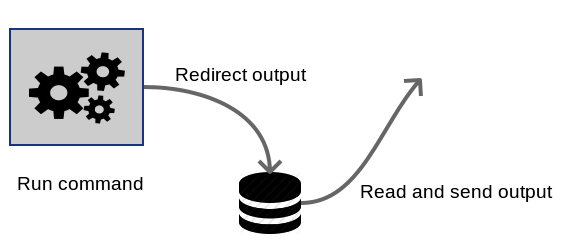
\includegraphics[scale=0.5]{Figures/local_exec.png}
    \rule{25em}{0.5pt}
  \caption[Local command execution]{Local execution on the slave node}
  \label{fig:local_exec}
\end{figure}


% --------------

\section{Varying the number of nodes}

An important aspect of distributed software of any kind is scalability - what is the relation between performance and number of nodes? Naturally, this is relevant for MTC filesystems as well. To measure this, we need to run the same benchmark on different numbers of nodes and then compare the results.

Since this is a given in MTC filesystem benchmarking, our solution handles this by default. The user can configure on what series of node numbers they want the test to run, and the benchmark will measure scalability automatically. To achieve this, we re-run the benchmark with more and more of the available nodes and keep track of the results.

\begin{figure}[H]
  \centering
    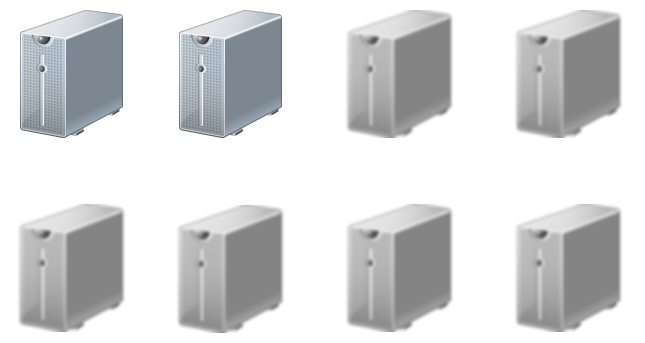
\includegraphics[scale=0.5]{Figures/nodes_grayed.png}
    \rule{25em}{0.5pt}
  \caption[Varying the number of nodes]{Varying the number of nodes}
  \label{fig:nodes_grayed}
\end{figure}

The implementation consists of a Python wrapper over the MPI code mentioned in Section~\ref{sec:coordination}. It iterates over an array of integers representing node counts and runs the benchmark with the given amount of nodes. Because it uses the MPI code, it needs to tell MPI exactly what nodes to use. This is done using a machinefile - a text file that contains node IPs, one per line. The MPI program always uses the same machinefile, and the Python wrapper updates it between runs as necessary, increasing the number of nodes.

Because clusters usually have a reservation process that a user has to go through before having access to a set of nodes, we added support for that to our solution as well. For this, we provide a \textit{reserve.sh} script that takes a number of nodes as argument and reserves that many nodes on the cluster. It also checks if the user already has reserved nodes and if so, it reuses those. The Python wrapper uses this script to reserve the maximum amount of nodes needed at the beginning of the run, and then uses them increasingly as the tests advance. So, if the user specified the array \textit{[1, 2, 4, 8, 16]} for the amounts of test nodes, the benchmark would reserve 16 nodes from the start and then run the tests with 1, 2, 4 (and so on) nodes.

The reason for which we kept the node reservation process in a separate script is that other clusters might require different commands to reserve nodes. We want our solution to be accessible to as many users as possible, and running on a different cluster shouldn't imply changing the benchmark's code. This way, the only necessary change is to adapt the \textit{reserve.sh} script.

In order to properly support multiple nodes in tests, there also needs to be a way to parametrize the given commands by nodes. For example, maybe the user wants node 3 to run IOzone against \texttt{test\_file\_3}. To achieve this, our tool sets an environment variable to the ID of every node, such that examining \texttt{\$\{NODENAME\}} on node 3 will yield \texttt{3}.

% ----------

\section{Leveraging existing benchmarks}

\begin{figure}[H]
  \centering
    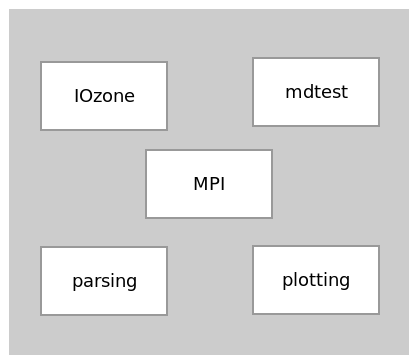
\includegraphics[scale=0.5]{Figures/components.png}
    \rule{25em}{0.5pt}
  \caption[Components]{Components}
  \label{fig:components}
\end{figure}

\subsection{IOzone}

% --------

\subsection{mdtest}

% --------




\subsection{Producing structured results}


\begin{figure}[H]
  \centering
    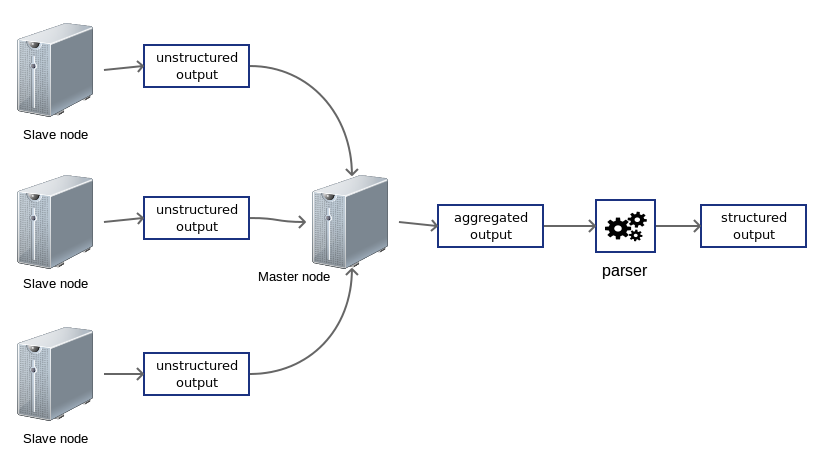
\includegraphics[scale=0.5]{Figures/output_flow.png}
    \rule{25em}{0.5pt}
  \caption[Flow of output through the system]{Flow of output through the system}
  \label{fig:output_flow}
\end{figure}

% ---------

\subsection{Plotting the results}


% --------

% ---------------


\section{Specifying complex test cases}

% TODO - sample listing with a test pseudocode

% --------------


\section{Putting it all together}

\begin{figure}[H]
  \centering
    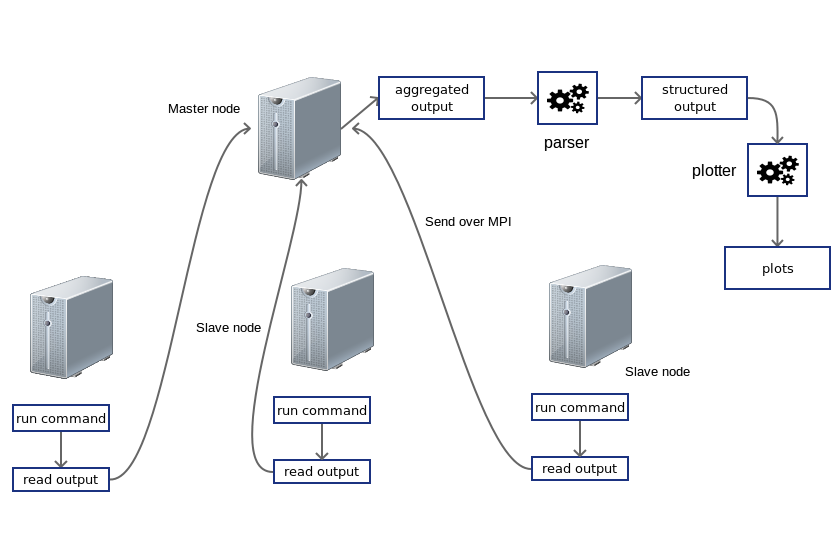
\includegraphics[scale=0.5]{Figures/architecture.png}
    \rule{25em}{0.5pt}
  \caption[General architecture]{General architecture}
  \label{fig:architecture}
\end{figure}


% ------------

% Chapter Template

\chapter{Evaluation} % Main chapter title

\label{Chapter4} % Change X to a consecutive number; for referencing this chapter elsewhere, use \ref{ChapterX}

\lhead{Chapter 4. \emph{Evaluation}} % Change X to a consecutive number; this is for the header on each page - perhaps a shortened title

To evaluate our solution, we follow two directions. First, we test the fact that our benchmark supports MTC filesystems and that it can measure the metrics described by the MTC Envelope. Second, we observe whether our project is easier to use than the current benchmarking solutions for MTC filesystems.

To assess the first part, we ran the following benchmarks on the two discussed MTC filesystems - MemFS and AMFS.

\begin{itemize}

\item 1-to-1 read
\item N-to-1 read
\item mdtest suite

\end{itemize}

All the tests were run on the following numbers of nodes: \texttt{[1, 2, 4, 8, 16, 32]}. The benchmarks were run on the DAS-4 cluster, using OpenMPI.

The N-to-1 access pattern was simulated using a test file such as the following:\\\\

\lstinputlisting[caption=Sample test file]{Files/test_example2.json}

Having this file stored as \textit{test.json}, we can run the benchmark with:

\begin{verbatim}
./dfs_bench.py --file test.json
\end{verbatim}

The full set of results can be found in the Appendix. However, we include here a sample results file and a plot to show the outputs of our benchmark.

The following listing represents a part of a results file of an IOzone-based benchmark, testing N-to-1 read. It depicts the processed result set for the test run with 2 nodes.

\begin{verbatim}
{
  "2": {
    "total": {
      "re-reader": 1433371, 
      "reader": 1345494
    }, 
    "individual": [
      {
        "re-reader": 728699, 
        "reader": 721448
      }, 
      {
        "re-reader": 704672, 
        "reader": 624046
      }
    ]
  }
}
\end{verbatim}

Based on a processed set of results, the \textit{make\_bar\_plots.py} script creates a plot like the following.

\begin{figure}[H]
  \centering
    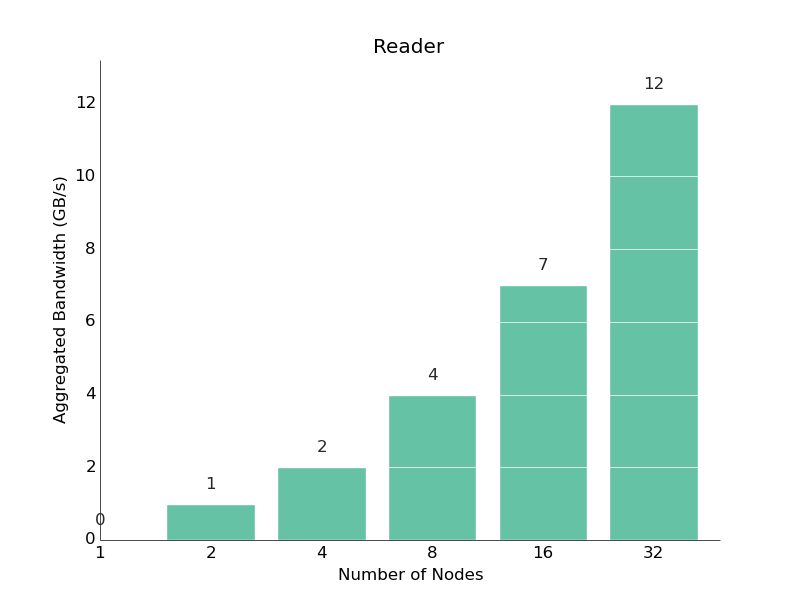
\includegraphics[scale=0.5]{Figures/reader.png}
    \rule{25em}{0.5pt}
  \caption[Generated sample plot]{Generated sample plot}
  \label{fig:architecture}
\end{figure}

we can see .. just one command , scaling taken care of, coordination, aggregation, plots
 
% Chapter Template

\chapter{Conclusions} % Main chapter title

\label{Chapter5} % Change X to a consecutive number; for referencing this chapter elsewhere, use \ref{ChapterX}

\lhead{Chapter 5. \emph{Conclusions}} % Change X to a consecutive number; this is for the header on each page - perhaps a shortened title

 
%\input{Chapters/Chapter6} 
%\input{Chapters/Chapter7} 

%----------------------------------------------------------------------------------------
%	THESIS CONTENT - APPENDICES
%----------------------------------------------------------------------------------------

\addtocontents{toc}{\vspace{2em}} % Add a gap in the Contents, for aesthetics

\appendix % Cue to tell LaTeX that the following 'chapters' are Appendices

% Include the appendices of the thesis as separate files from the Appendices folder
% Uncomment the lines as you write the Appendices

% Appendix A

\chapter{Example Test Files and Commands} % Main appendix title

\label{AppendixA} % For referencing this appendix elsewhere, use \ref{AppendixA}

\lhead{Appendix A. \emph{Example Test Files and Commands}} % This is for the header on each page - perhaps a shortened title

\lstinputlisting[caption=Test file for 1 to 1 read]{Files/test_example.json}

\lstinputlisting[caption=Test file for N to 1 read]{Files/test_example2.json}

\begin{lstlisting}[caption=Running benchmark from a file]
./dfs_bench.py --file test_example.json
\end{lstlisting}

\begin{lstlisting}[caption=Running 1 to 1 read benchmark directly]
./dfs_bench.py './iozone -f /var/scratch/mdr222/${NODENAME}_test -S 12000 -L 64 -c -e -s 1M -i0 -i1 -r 128 -R'
\end{lstlisting}

\begin{lstlisting}[caption=Running mdtest]
./run_mdtest.py 'mdtest -C -i 10 -n 100 -S -d /local/aua400/kvstore'
\end{lstlisting}

%% Appendix A

\chapter{Example Plots} % Main appendix title

\label{AppendixB} % For referencing this appendix elsewhere, use \ref{AppendixA}

\lhead{Appendix B. \emph{Example Plots}} % This is for the header on each page - perhaps a shortened title

\begin{figure}[H]
  \centering
    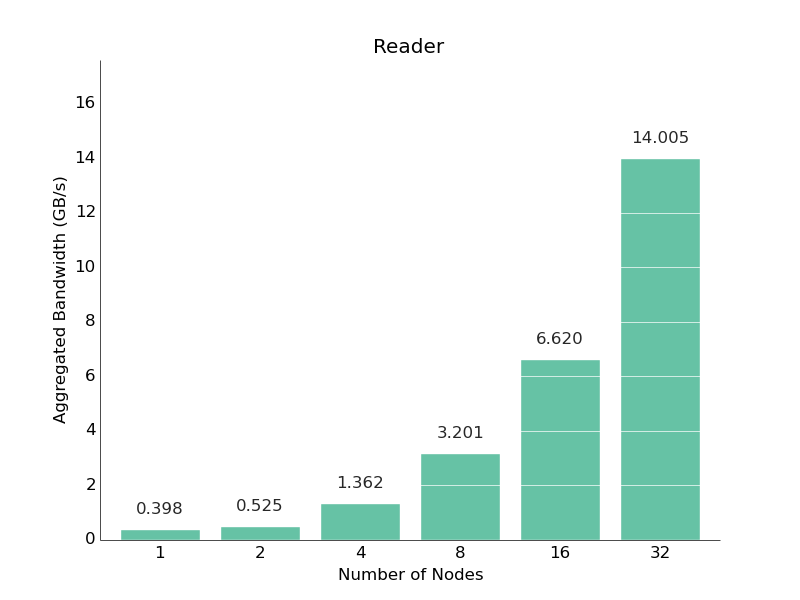
\includegraphics[scale=0.6]{Figures/amfora_32_n_to_1.png}
    \rule{25em}{0.5pt}
  \caption[AMFS, N-to-1 read]{AMFS, N-to-1 read}
  \label{fig:plot1}
\end{figure}

\begin{figure}[H]
  \centering
    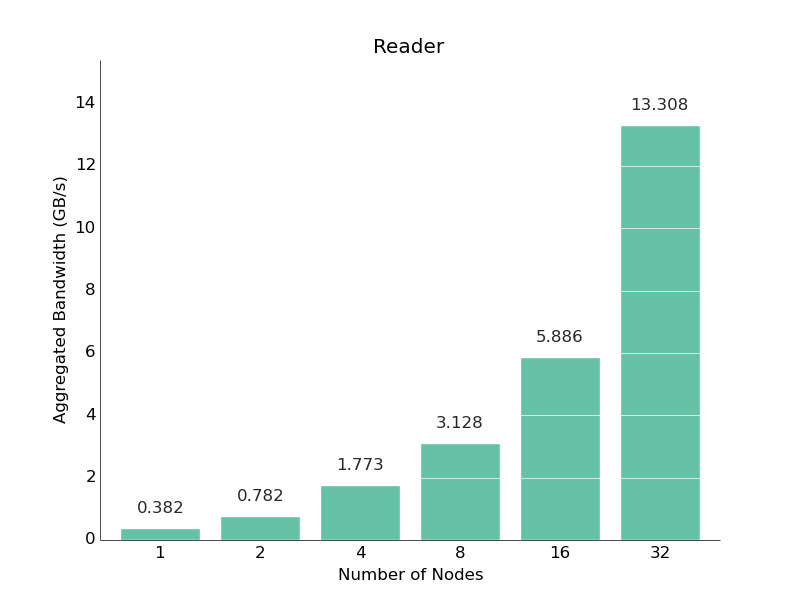
\includegraphics[scale=0.6]{Figures/amfora_32_1_to_1.png}
    \rule{25em}{0.5pt}
  \caption[AMFS, 1-to-1 read]{AMFS, 1-to-1 read}
  \label{fig:plot2}
\end{figure}

\begin{figure}[H]
  \centering
    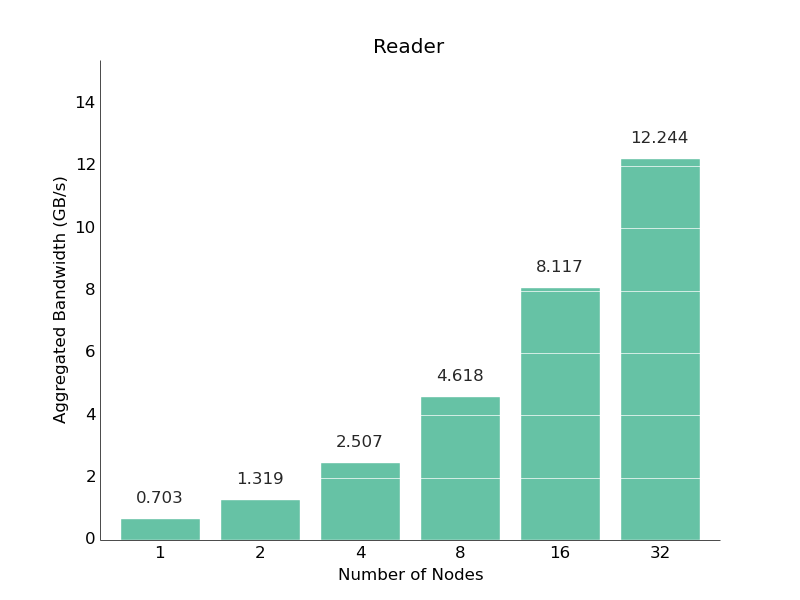
\includegraphics[scale=0.6]{Figures/memfs_32_1_to_1.png}
    \rule{25em}{0.5pt}
  \caption[AMFS, N-to-1 read]{MemFS, N-to-1 read}
  \label{fig:plot3}
\end{figure}

\begin{figure}[H]
  \centering
    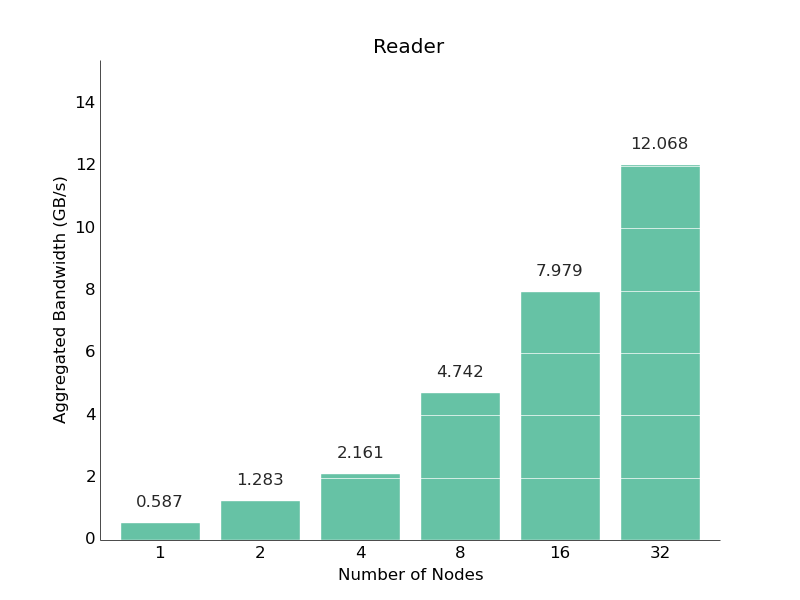
\includegraphics[scale=0.6]{Figures/memfs_32_N_to_1.png}
    \rule{25em}{0.5pt}
  \caption[AMFS, N-to-1 read]{MemFS, 1-to-1 read}
  \label{fig:plot4}
\end{figure}

% TODO - mdtest plots
%\input{Appendices/AppendixC}

\addtocontents{toc}{\vspace{2em}} % Add a gap in the Contents, for aesthetics

\backmatter

%----------------------------------------------------------------------------------------
%	BIBLIOGRAPHY
%----------------------------------------------------------------------------------------

\label{Bibliography}

\lhead{\emph{Bibliography}} % Change the page header to say "Bibliography"

\bibliographystyle{unsrtnat} % Use the "unsrtnat" BibTeX style for formatting the Bibliography

\bibliography{Bibliography} % The references (bibliography) information are stored in the file named "Bibliography.bib"

\end{document}  